\documentclass{beamer}


\usepackage{amsmath}
\usepackage{amsthm}
\usepackage{amsfonts}

\usepackage{accents}
\usepackage{graphicx}
\def\b{\begin}
\def\e{\end}
\def\tb{\textbf}
\def\p{\partial}
\def\CC{\mathbb{C}}
\def\f{\frac}
\def\RR{\mathbb{R}}


\theoremstyle{plain}
\newtheorem{prop}{Proposition}
\newtheorem{thm}{Theorem}[section]
\newtheorem{claim}{Claim}
\newtheorem{lem}[thm]{Lemma}

\theoremstyle{definition}
\newtheorem{dfn}{Definition}[section]




\begin{document}

\title{\textbf{Uncertainty of Rogue Wave Formation in the Nonlinear Schr\"{o}dinger Equation}}
\author{\textsc{by Andy Reagan}}
\date{October 2, 2012}


\frame{\maketitle}



\section[Outline]{}
\frame{\tableofcontents}

\section{Introduction: Rogue Waves}

\frame
{
\begin{figure}
\begin{center}
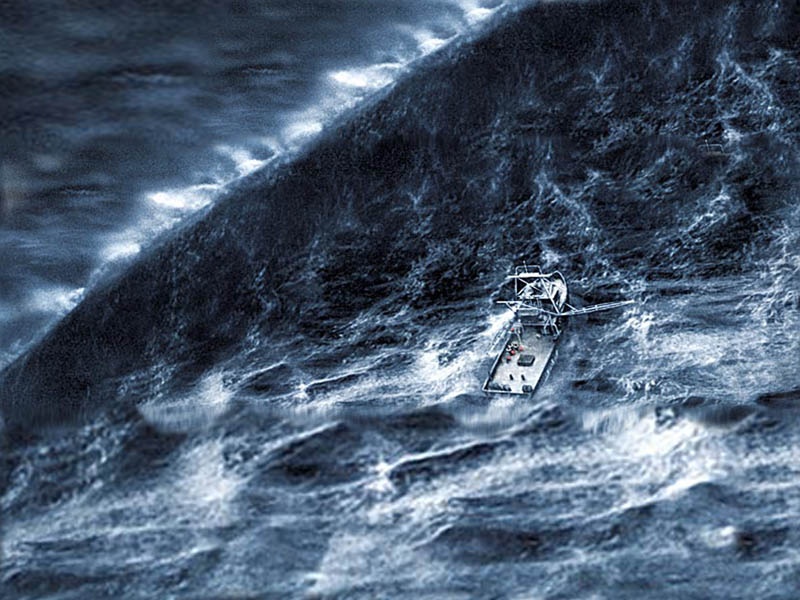
\includegraphics[width=200px]{perfect-storm.jpeg}\\
Figure 0: Rogue wave?
\end{center}
\end{figure}
\vspace{-1mm}
}

\frame
{
\begin{figure}
\begin{center}
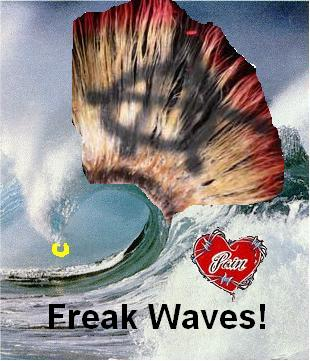
\includegraphics[width=200px]{reardon.JPG}\\
Figure 1: Definitely rogue
\end{center}
\end{figure}
\vspace{-1mm}
}

\frame
{
\begin{figure}
\begin{center}
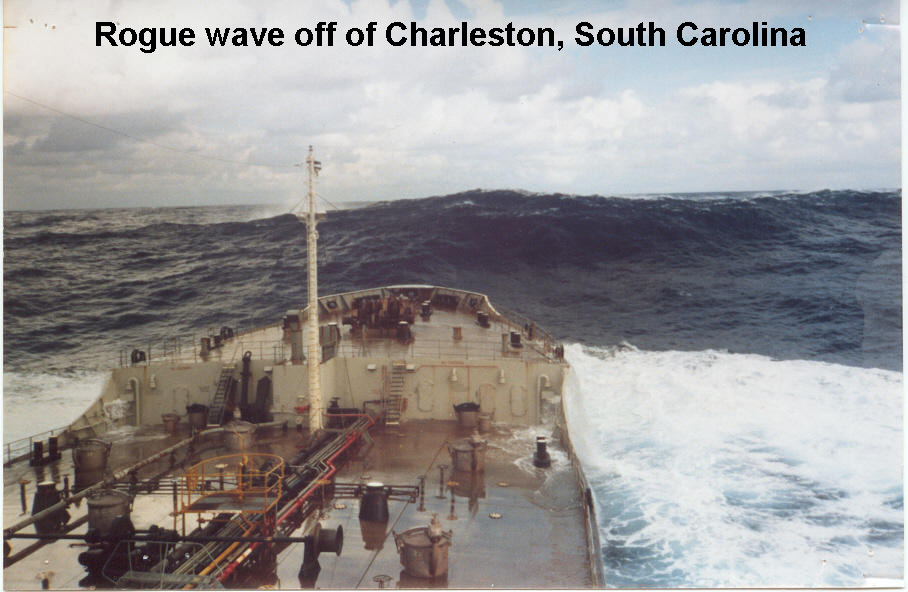
\includegraphics[width=200px]{rogue_wave2.jpg}\\
Figure 2: Observed rogue wave
\end{center}
\end{figure}
\vspace{-1mm}
}
  
  
 \frame
{
\begin{figure}
\begin{center}
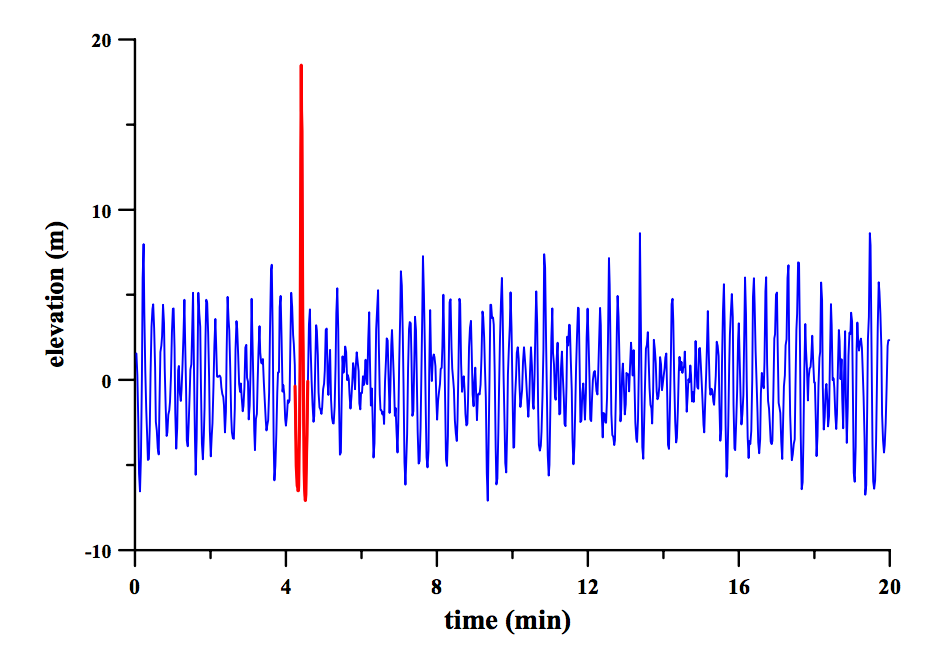
\includegraphics[width=200px]{draupner_wave.png}\\
Figure 3: The "Draupner Wave"
\end{center}
\end{figure}
\vspace{-1mm}
}
  

\frame{  
\frametitle{What are rogue waves}
\b{itemize}

\item Once considered to be a mythical occurrence, rogue waves are now a studied phenomenon in nonlinear wave  theory. \\[25pt]

\pause
\item The structure and nature of these waves is imperative in our understanding of how and why they occur.\\[25pt]

\pause
\item Occur in both water and optical waves.
\e{itemize}
}

\frame
{
\b{itemize}
\item In oceanography, the pragmatic approach is to 
define a rogue wave whenever
\begin{equation*}\tag{1.1}
H/H_s>2\quad\text{or}\quad\omega_c/H_s>1.25
\e{equation*}
where $H$ is the wave height (distance from trough to crest), $\omega_c$ is the crest height (distance from mean sea level to crest), and $H_s$ is the significant wave height, here defined as four times the standard deviation of the surface elevation.

\pause
\item Known to cause extensive damage, and are even life-threatening, when they come into contact with ocean liners and passenger ships in the open waters.  

\pause
\item Between 1964 and 1994, it is estimated that more than 22 super-carriers have been lost at sea as a direct result of rogue waves (Kharif \& Pelinovsky 2003).
\e{itemize}
}

\frame
{
\frametitle{Physical mechanisms of rogue wave formation}
\b{itemize}

\item Normal part of wave spectrum\\[25pt]

\pause
\item Linear and non-linear spatial focusing\\[25pt]

\pause
\item Non-linear modulation instability

%\item Recently, there has been the discovery of a similar wave phenomenon observed in optics\\[10pt]
%\item A growing consensus is that both oceanic and optical rogue waves appear as a result of modulation instability of monochromatic nonlinear waves (Ohta \& Yang 2012). \\[10pt]
%\item As a result, we must turn to mathematically studying these waves thus we turn our attention to an integrable model, the nonlinear Schr\"{o}dinger (NLS) (Zakharov \& Shabat 1967). 
\e{itemize}
}

\frame
{
\frametitle{Rogue Wave Models}
\b{itemize}
\item Deep water waves described by NLS: $$iu_t + u_{xx} + 2|u|^2u = 0$$\\[5pt]

\pause
\item Rogue wave like solution first discovered by Peregrine in 1983\\[25pt]

\pause
\item This Peregrine Soliton is a first order rational soliton, and limiting case of the known Akmediev and Ma breathers

\e{itemize}
}

\frame
{
\frametitle{}

\begin{figure}
\begin{center}
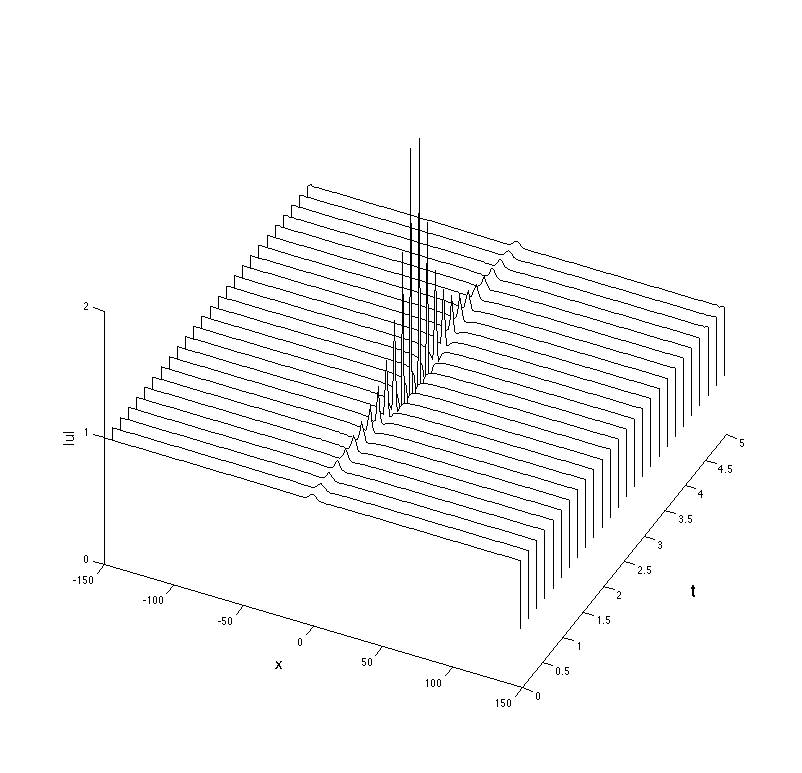
\includegraphics[width=220px]{peregrine_4096pts_256plotted_0eps.png}\\
Figure 4: The Peregrine Soliton
\end{center}
\end{figure}


}

\section{Introduction: Uncertainty Quantification}

\frame
{
\frametitle{UQ}
\b{itemize}
\item Goal: characterize and control uncertainty in model output propagated from uncertain input\\[25pt]

\pause
\item Methods:
\b{itemize}
\item Monte Carlo sampling\\[5pt]
\item Polynomial chaos expansions\\[5pt]
\item Most probable point methods\\[5pt]
\item Perturbation method\\[5pt]
\item Dimension reduction
 
\e{itemize}
\e{itemize}
}

\frame
{
\frametitle{Example UQ Problems}
\b{itemize}
\item Broad: weather prediction
\begin{figure}
\begin{center}
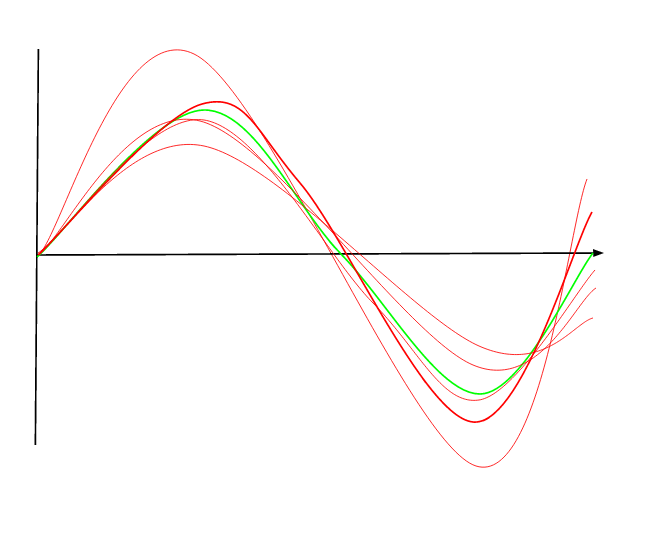
\includegraphics[width=100px]{UQ_weather.png}
\end{center}
\end{figure}

\pause
\item Specific: recovering flight data from HyShot II experiment
\begin{figure}
\begin{center}
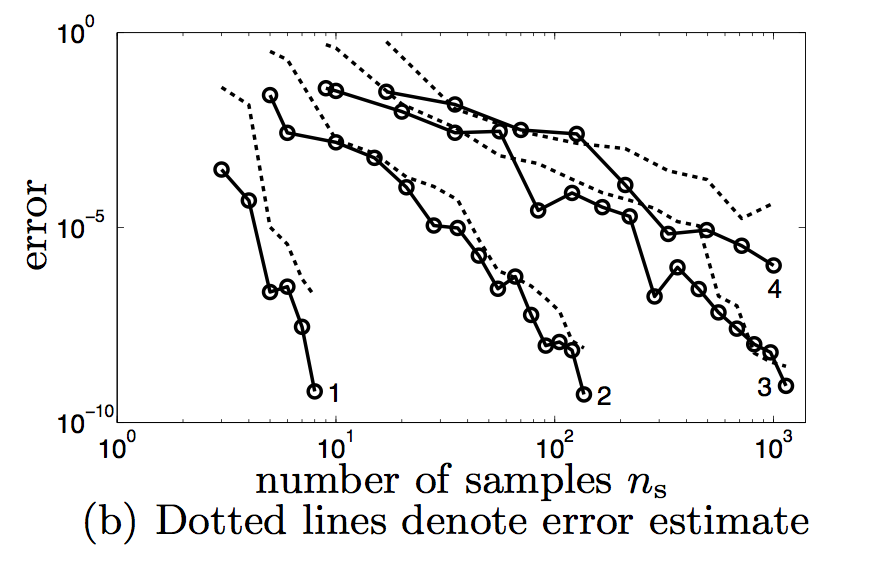
\includegraphics[width=100px]{UQ_hyshot.png}
\end{center}
\end{figure}
\e{itemize}
}



\section{Peregrine soliton formation under uncertain IC}

\frame
{
\frametitle{UQ of PS formation}
\b{itemize}
\item Want to characterize formation of PS with uncertain initial condition\\[25pt]

\pause
\item Can control parameters of noise\\[5pt]
\b{itemize}
\item Random (gaussian) noise: amplitude\\[5pt]
\item Superposition of random waves: steepness, wavelength, amplitude
 
\e{itemize}
\e{itemize}
}


%%%%%%%%%%%%%%%%%

%picture blast

\frame
{
\begin{figure}
\begin{center}
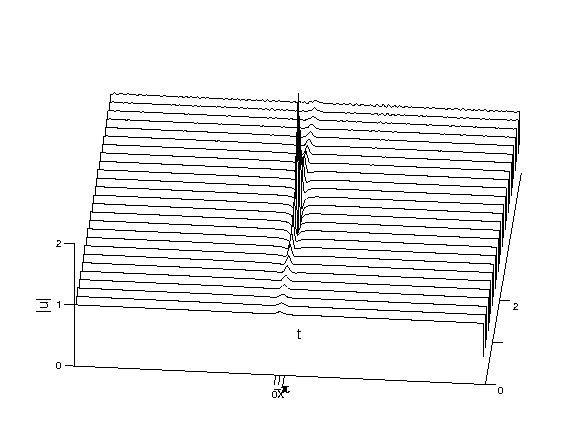
\includegraphics[width=250px]{peregrine_16384pts_256plotted_point0001eps.png}\\
peregrine 16384pts 256plotted point0001eps
\end{center}
\end{figure}
}

\frame
{
\begin{figure}
\begin{center}
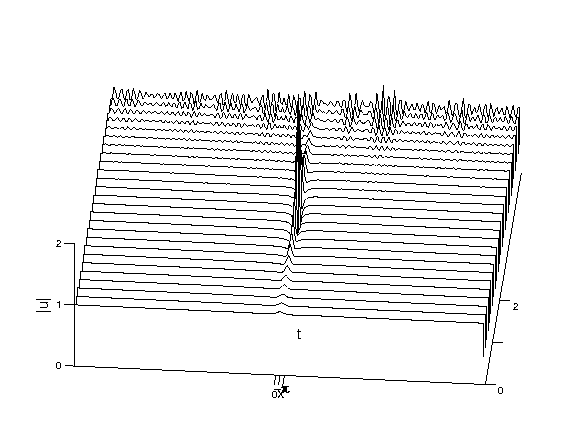
\includegraphics[width=250px]{peregrine_16384pts_256plotted_point001eps.png}\\
peregrine 16384pts 256plotted point001eps
\end{center}
\end{figure}
}

\frame
{
\begin{figure}
\begin{center}
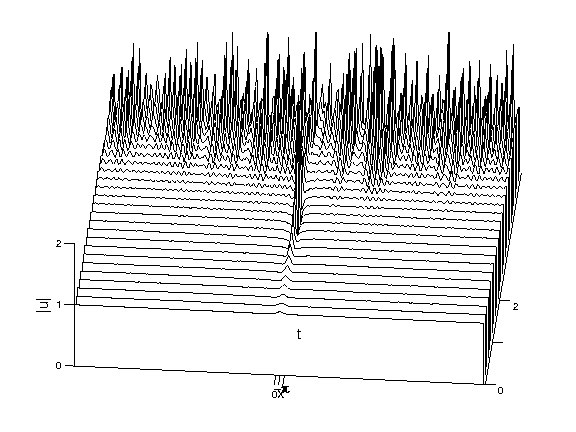
\includegraphics[width=250px]{peregrine_16384pts_256plotted_point01eps.png}\\
peregrine 16384pts 256plotted point01eps
\end{center}
\end{figure}
}

\frame
{
\begin{figure}
\begin{center}
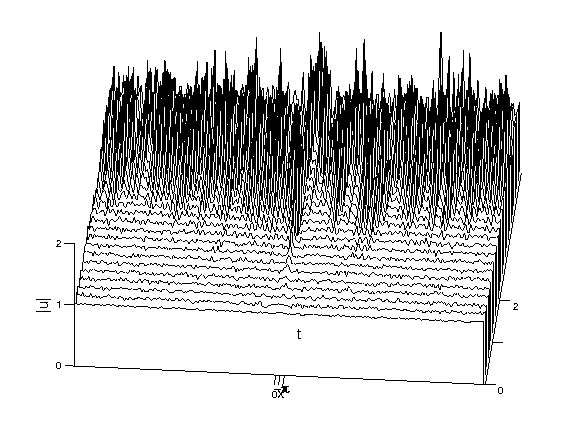
\includegraphics[width=250px]{peregrine_16384pts_256plotted_point1eps.png}\\
peregrine 16384pts 256plotted point1eps
\end{center}
\end{figure}
}

\frame
{
\begin{figure}
\begin{center}
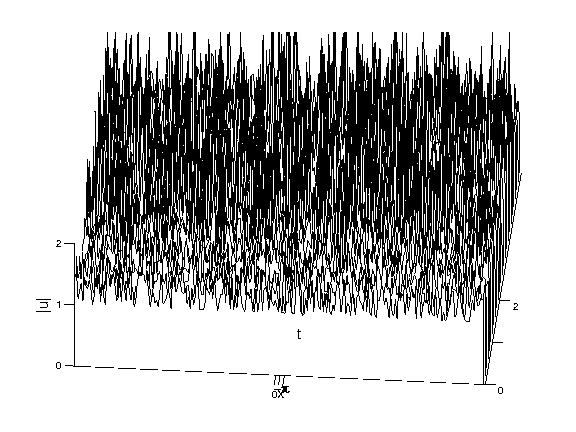
\includegraphics[width=250px]{peregrine_16384pts_256plotted_1eps.png}\\
peregrine 16384pts 256plotted 1eps
\end{center}
\end{figure}
}


\frame
{
\begin{figure}
\begin{center}
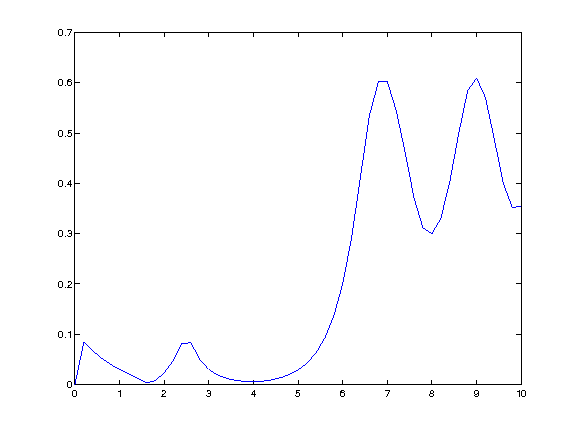
\includegraphics[width=250px]{16384pts_error_point0001eps_long.png}\\
16384pts error point0001eps long
\end{center}
\end{figure}
}

\frame
{
\begin{figure}
\begin{center}
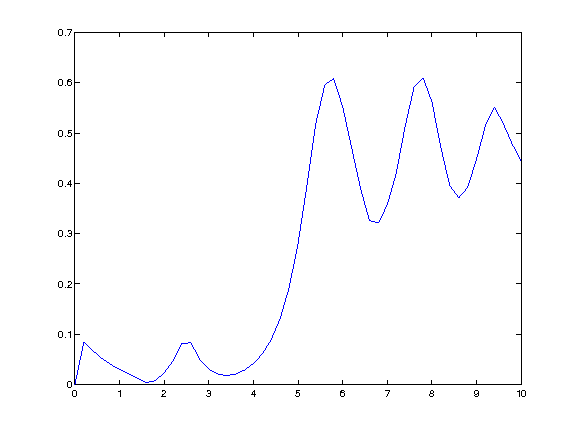
\includegraphics[width=250px]{16384pts_error_point001eps_long.png}\\
16384pts error point001eps long
\end{center}
\end{figure}
}

\frame
{
\begin{figure}
\begin{center}
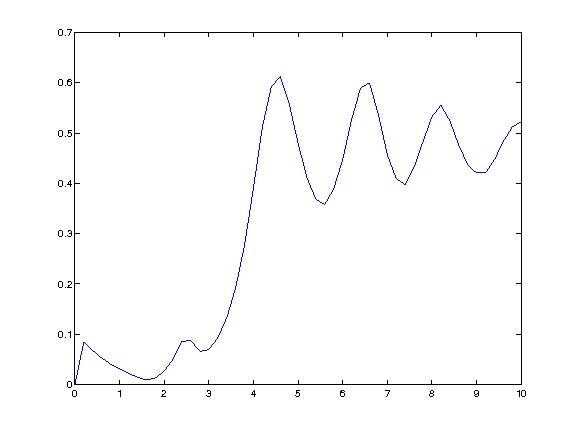
\includegraphics[width=250px]{16384pts_error_point01eps_long.png}\\
16384pts error point01eps long
\end{center}
\end{figure}
}

\frame
{
\begin{figure}
\begin{center}
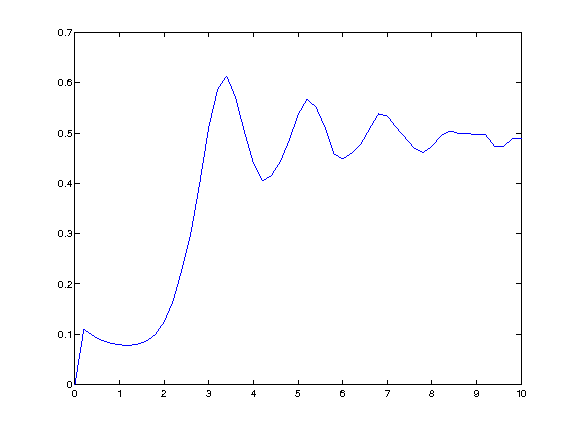
\includegraphics[width=250px]{16384pts_error_point1eps_long.png}\\
16384pts error point1eps long
\end{center}
\end{figure}
}

\frame
{
\begin{figure}
\begin{center}
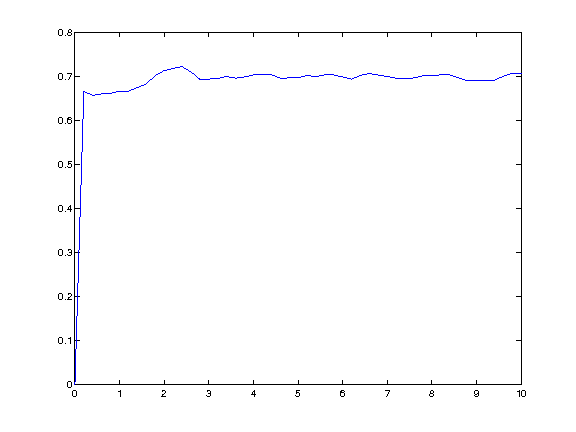
\includegraphics[width=250px]{16384pts_error_1eps_long.png}\\
16384pts error 1eps long
\end{center}
\end{figure}
}


\frame
{
\begin{figure}
\begin{center}
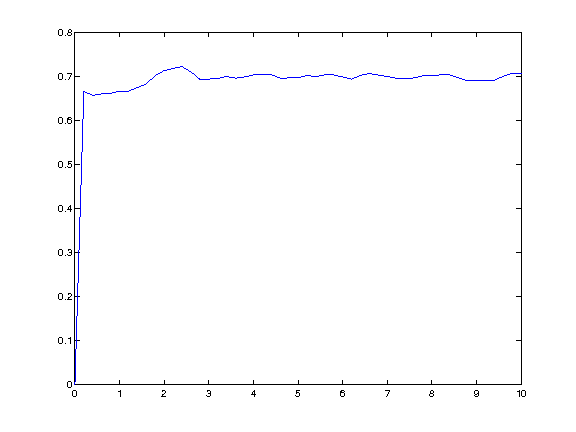
\includegraphics[width=250px]{16384pts_error_1eps_long.png}\\
16384pts error 1eps long
\end{center}
\end{figure}
}



\frame
{
\frametitle{Next steps}
\b{itemize}
\item Create error from wave superposition $$u^* = u + \epsilon \sum ^N e^{ik x} $$\\[25pt]

\pause
\item Extend to 3-Dimensional NLS\\[5pt]
\b{itemize}
\item With random wave superposition, look for parameters leading to more freak waves
 
\e{itemize}
\e{itemize}
}



\end{document}